\documentclass[11pt,a4paper]{article}
\usepackage{fontspec}
\setmainfont{NimbusRoman}[Extension=.otf,UprightFont=*-Regular,BoldFont=*-Bold,
  ItalicFont=*-Italic,BoldItalicFont=*-BoldItalic]
\setsansfont{NimbusSans}[Extension=.otf,UprightFont=*-Regular,BoldFont=*-Bold,
  ItalicFont=*-Italic,BoldItalicFont=*-BoldItalic]
\usepackage{amsmath,unicode-math}
\setmathfont{Latin Modern Math}
\usepackage[a4paper,left=20mm,right=20mm,top=20mm,bottom=20mm]{geometry}
\usepackage{graphicx,booktabs,tabularx,array,placeins,microtype}
\usepackage[font=small,labelfont=bf,labelsep=period,singlelinecheck=false]{caption}
\usepackage[hidelinks]{hyperref}
\renewcommand{\figurename}{Fig.}
\setlength{\parindent}{0pt}
\setlength{\parskip}{0.45em}
\setlength{\textfloatsep}{13pt}
\setlength{\intextsep}{11pt}
\setlength{\emergencystretch}{1em}
\hypersetup{pdftitle={Actuarial digital twins for heatwave accumulation in European power insurance},
  pdfauthor={Prashant Pant, Vladimir Terzija and Thomas Hamacher}}

\title{\bfseries Actuarial digital twins for heatwave accumulation in European power insurance}
\author{Prashant Pant\textsuperscript{1}, Vladimir Terzija\textsuperscript{2} and Thomas Hamacher\textsuperscript{1}\\[0.5em]
\small \textsuperscript{1}Technical University of Munich, Munich, Germany\quad
\textsuperscript{2}Newcastle University, Newcastle upon Tyne, UK}
\date{\small Research draft \textbar{} 12 November 2026}

\begin{document}
\maketitle
\begin{abstract}
A European heatwave can cause breakdowns at several sites within days, accumulating claims across a power insurer's portfolio. In ERA5, seven of ten pilot sites reached at least 4\,K above their local summer threshold during 17--21 July 2022, with at most four reaching it on any one day. We test an actuarial digital twin that supplies the same site condition estimate to the owner for targeting interventions and to the insurer for estimating covered loss. In an ERA5-calibrated simulation with assumed vulnerability and equipment-breakdown policies covering damage and consequent business interruption, twin-guided operation reduced median average annual covered loss by 37\% and the 99.5th-percentile annual loss by 13\% at matched intervention spending. Holding operation fixed, twin evidence reduced the insurer's tail-estimation error from 30.2\% to 7.5\% RMSE. The design distinguishes claims avoided through intervention from improvements in estimating the remaining exposure.
\end{abstract}

\section*{Introduction}

Heatwaves can stress geographically dispersed power assets over several days. A transformer, inverter or battery system can reach its thermal limit as loading and heat-rejection conditions change. If several sites break down during the same spell, repair costs and business interruption accumulate across the insurer's portfolio. The heat forecast describes which sites are exposed, while the state of each asset helps determine where an intervention can reduce the chance of breakdown.

The owner and insurer use this information for different decisions. The owner can act before the forecast heat arrives, for example by transferring load or limiting inverter output. The insurer must estimate the covered losses remaining after those actions, including their concentration in severe years. An actuarial digital twin (ADT) links the engineering estimate of site condition to failure, restoration and policy response \cite{aes}. Prior work in DT-INSURE and SPARC develops these links for PV inverters and battery storage \cite{dtinsure,sparc}. The question here is what changes when the same regional heatwave exposes several sites together.

We use European ERA5 data to examine the timing and geographic reach of heat, then test two uses of the same condition estimate in a simulated portfolio. For the owner, we compare twin-guided and class-based operating rules at matched intervention spending. For the insurer, we hold the operating rule fixed and compare class evidence with site-level twin evidence. We model equipment breakdown with physical damage and resulting business interruption (BI), a combination available in operational power insurance \cite{hsb,chubb}. The loss model uses assumed vulnerability and terms. The European inverter field analysis informs which parts of the engineering chain can be checked with telemetry.

\section*{Results}

\subsection*{Heat exposure spans several sites over successive days}

Seven of the ten sites reached a daily maximum at least 4\,K above their local June--August 90th percentile during 17--21 July 2022 (Fig.~\ref{fig:weather}a). At most four reached that threshold on the same day. Exceedances within that window extend from Almaraz in western Spain to Bełchatów in central Poland (Fig.~\ref{fig:weather}b shows the daily counts). The rate of spells peaking above 4\,K increased from 0.37 to 0.72 per site-year between 1991--2005 and 2011--2025 (55 and 108 spells across ten sites in the respective periods, Fig.~\ref{fig:weather}c). This is a descriptive comparison for the selected sites. The daily sequence shows why a definition of the event window matters when modelling claims accumulation.

\begin{figure}[htbp]
\centering
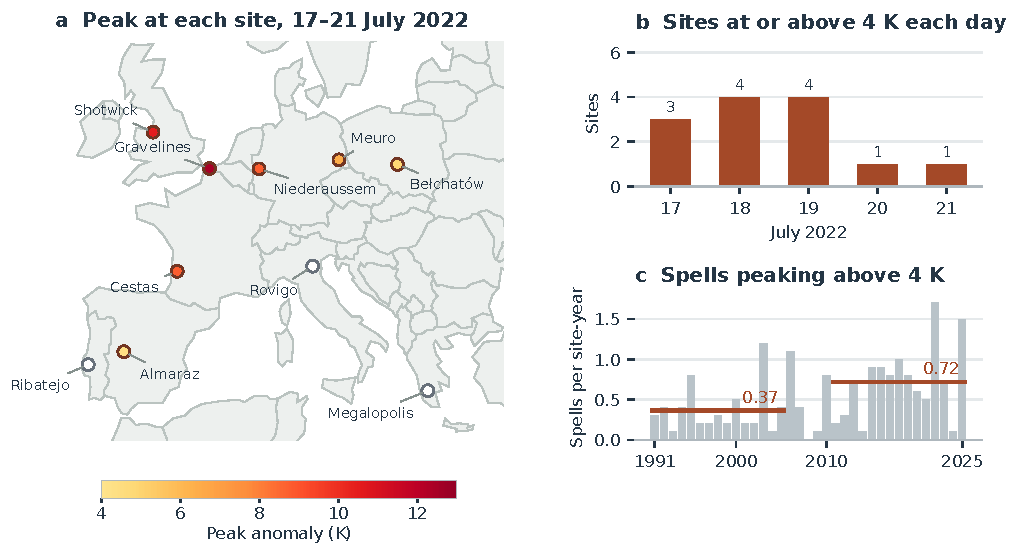
\includegraphics[width=\linewidth]{figures/era5_observed.pdf}
\caption{\textbf{European heat exposure during 17--21 July 2022.}
\textbf{a}, Peak daily maximum air-temperature anomaly at each of ten sites over the five-day window, relative to its 1991--2020 June--August 90th percentile. Symbols show site values and open markers indicate a peak below 4\,K. The maxima may occur on different days.
\textbf{b}, Number of sites at or above 4\,K on each day.
\textbf{c}, Annual count of site spells peaking above 4\,K, divided by ten. Orange segments show the two period means. A site spell lasts at least three consecutive days above its baseline.}
\label{fig:weather}
\end{figure}

The generator reproduces the broad pattern of spell frequencies but its fitted dependence is imperfect. For a site spell peaking at or above 4\,K, the fraction of neighbouring peaks reaching at least half that anomaly is 25\% in ERA5 and 14\% in the model for distances of 800--1,300\,km. The observed statistic uses a three-day window around the focal site's peak. The model assigns a shared peak day within each event. Gridded daily histories would allow direct testing of the spatial extent and timing used to aggregate site losses.

\subsection*{One twin informs two decisions}

The engineering twin estimates \emph{thermal headroom}, the ambient heat anomaly that would bring a site to its thermal limit at a given operating point. Owners compare that estimate with the heat forecast to decide where to intervene (Fig.~\ref{fig:workflow}). In the simulation an action temporarily adds headroom at a cost. A class-based rule uses a common estimate within each asset class. A twin-guided rule uses the site estimate to direct intervention towards assets closer to their limit.

The insurer uses the same condition estimate to update its class-based assessment of headroom while retaining regional dependence. It then applies the owner's operating rule and the policy terms to estimate the distribution of covered claims. An action log matters because the frequency of breakdowns reflects the interventions taken as well as the underlying condition. A shared record of actions, failures, restoration and claims would let the insurer check how much reliance the twin merits on the covered-loss outcome \cite{aes}.

\begin{figure}[htbp]
\centering
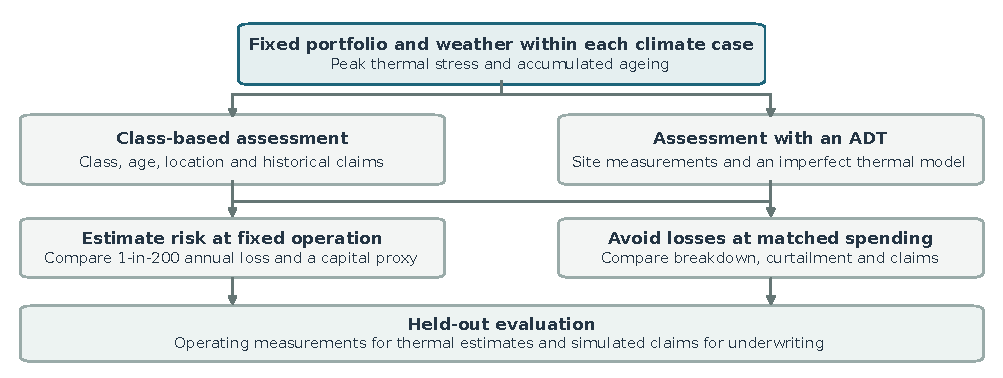
\includegraphics[width=\linewidth]{figures/adt_workflow.pdf}
\caption{\textbf{An actuarial digital twin shared by owner and insurer.}
The owner uses site headroom and the forecast to target actions. The insurer models claims under the resulting operating rule. The shared record supplies evidence to validate both the operating response and the insurer's reliance on twin information.}
\label{fig:workflow}
\end{figure}

\subsection*{Targeted operation reduces average loss more than tail loss}

We simulate ten portfolios with the same exposure, vulnerability and contract in each paired comparison. At matched mean intervention spending, twin-guided operation reduces average annual covered loss by a median of 37\% (book range 23--55\%) and 99.5th-percentile annual covered loss by 13\% (7--27\%) (Fig.~\ref{fig:loss}a). The comparison with a class rule using the same trigger margin yields a 58\% average-loss reduction and a 25\% tail reduction, with median intervention spending 70\% higher for twin-guided operation. At matched spending, the median tail benefit across four paired books falls from 15\% under the base calibration to 9\% under the heavier-tail variant. In the model, each action adds a finite amount of headroom that severe heat can still exceed. The heavier-tail check shows how much the estimated benefit depends on the event generator.

\subsection*{Condition evidence improves the insurer's estimate of the remaining tail}

Holding the class-based operating rule fixed, we then change only the information used to estimate headroom in underwriting. The relative 99.5th-percentile loss error across the ten synthetic books has an RMSE of 30.2\% with class evidence and 7.5\% with twin evidence (Fig.~\ref{fig:loss}b). The comparison is against the simulated loss for each book. With this operating rule, the median fraction of simulated years exceeding the modelled threshold changes from 0.18\% with class evidence to 0.60\% with twin evidence, against the nominal exceedance probability of 0.50\%. A smaller estimation error can bring funding closer to its target while increasing exceedances in books for which the class estimate was conservative.

\begin{figure}[htbp]
\centering
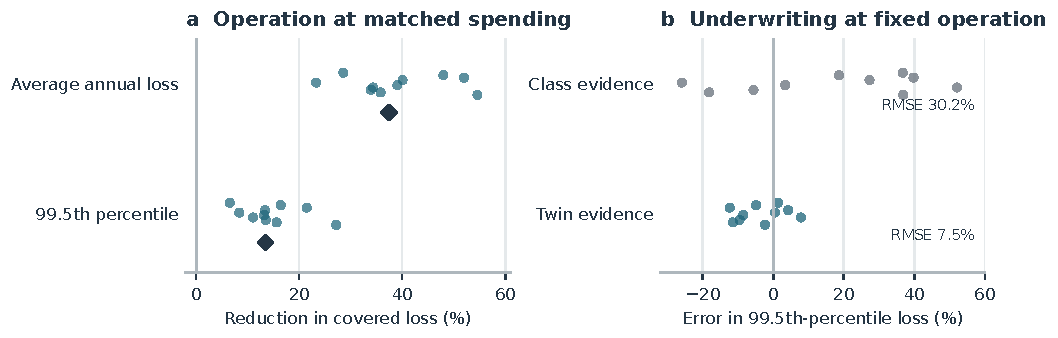
\includegraphics[width=\linewidth]{figures/era5_simulated_losses.pdf}
\caption{\textbf{Simulated effects of condition information.}
\textbf{a}, Reduction in covered loss with twin-guided operation relative to a class rule matched on average intervention spending. Dots represent synthetic books and diamonds mark medians.
\textbf{b}, Relative error in annual 99.5th-percentile covered loss against simulated loss for the same book, holding class-based operation fixed. RMSE is across books. The panels use the base ERA5-calibrated event generator and the assumed breakdown contract in Table~\ref{tab:terms}.}
\label{fig:loss}
\end{figure}

\FloatBarrier
\section*{Discussion}

The European heat footprint explains why site-level decisions have to be evaluated at portfolio scale. Intervening where thermal headroom is small can avoid a large share of ordinary breakdown losses in the simulation. Severe heat can exceed the extra headroom at several sites, leaving a substantial residual tail. Estimating that tail is a separate task for the insurer. The same-book comparison shows how condition evidence can improve its estimate even when the operating rule is fixed.

The benefit to each party depends on its exposure. Owners face intervention costs, retained damage and uninsured generation losses. Insurers face covered claims under the policy. A premium adjustment changes how the financial benefit is shared between them. Evidence for a renewal decision would need to link the action taken, the physical outcome, downtime and the actual claim, with an out-of-sample test of the improvement in covered-loss estimates \cite{aes}. The 35-year, ten-site weather sample leaves substantial uncertainty about the extent and intensity of rare heatwaves.

The field evidence supports parts of this chain. The Bali case in DT-INSURE demonstrates inverter thermal modelling with SCADA data \cite{dtinsure}. In North Macedonia, internal inverter temperature modestly improves forecasts of self-derating, while the model underestimates coincident starts (Extended Data Fig.~1). These observations concern reversible operating states. Confirming heat-related breakdown and consequent BI requires fault causes, repair records, the effect on plant delivery and the policy schedule. SPARC provides a design for estimating cause-specific severity and testing shared causes before aggregating losses \cite{sparc}.

Golfech illustrates a separate mechanism. EDF shut down unit 1 in June 2025 ahead of a forecast rise in Garonne river temperature \cite{golfech}. Modelling this type of curtailment requires site-specific cooling-water conditions and operating limits. A separate weather-index analysis can assess how such non-damage production losses might be transferred. The results here concern physical breakdown and resulting BI.

\section*{Methods}

\subsection*{Historical heat and event calibration}

We use ERA5 daily maximum 2\,m air temperature at ten WRI plant locations from 1991 to 2025. The sites were selected by country and technology strata for a data pilot. The repository records the grid cells, daily UTC aggregation and extraction settings \cite{era5,heatwave}. For each site, we subtract its 1991--2020 June--August 90th percentile and identify runs of at least three consecutive May--September days with a positive anomaly. The July footprint uses the maximum at each site over a five-day window centred on 19 July. Period comparisons count local spells with peaks strictly above 4\,K. The dependence diagnostic compares a focal spell peak at or above 4\,K with the largest anomaly at each other site within one day of its peak, with ratios clipped to the modelled range.

The synthetic generator uses Poisson event counts, stationary elliptical footprints and a generalised Pareto distribution for the anomaly at each event centre. Simulated moments fit the site-level rates of peak anomalies and distance-binned co-exceedance to the ten-site ERA5 sample. The base fit has about 7.64 events per simulated year and a fitted upper endpoint of 13.1\,K at the event centre. The heavier-tail sensitivity uses an endpoint of 15.6\,K. Both are properties of the fitted distributions. Event duration and normalised profiles are resampled from observed local spells in three peak-intensity classes and applied across the footprint. Regional event-centre weights remain assumed, and the stationary footprint cannot represent movement over days.

\subsection*{Inverter observations}

We use the FusionSolar records in SolarMagix v2 for January--May 2025. Self-derating starts are defined from the vendor state code on the five-minute sampling grid. The weather-and-load and condition models are fitted on January--April and tested on May from the same fleet. Both include plant and unit effects, operating state, recent output and weather. The condition model also uses current internal temperature and a residual from a thermal reference model. Observed fleet counts and expected counts under two dependence structures use the same eligible windows and unit probabilities \cite{observed}. The record covers 37 inverters at six plants and includes 969 bounded self-derating episodes, with a median duration of ten minutes. On the May holdout, adding internal temperature and the thermal residual reduces five-minute onset log loss from 0.01166 to 0.01133. The condition model predicts about 735 starts, with 738 observed. Two plants contribute 736 starts, and outdoor air temperature in the monitored fleet reaches 27\,°C. Extended Data Fig.~1 compares coincident starts on this holdout.

\subsection*{Portfolio, breakdown and restoration}

Each synthetic book contains 120 utility PV sites, 80 grid transformers, 40 battery storage sites and 25 thermal plants. Each site has a fixed thermal headroom in the simulation, built from a class mean and correlated regional and site terms. The twin estimate adds assumed measurement error. Forecast errors have shared event and site components. A site receives an intervention when its forecast anomaly exceeds the estimated headroom less a trigger margin. The intervention temporarily adds class-specific headroom and incurs a daily cost. For the matched-spending comparison, the class margin is set on the same event sample used for evaluation. Independent evaluation and optimisation of both decision rules remain needed.

Let \(x_{iek}\) be positive exceedance above effective headroom at site \(i\), event \(e\) and day \(k\). The prototype probability of physical breakdown for that site and event is
\[
p_{ie}=1-\exp\!\left[-\lambda_{0,c}\sum_k
  \left(2^{x_{iek}/\theta_c}-1\right)\right],
\]
with assumed class-specific parameters \(\lambda_{0,c}\) and \(\theta_c\).
When the simulation draws a breakdown, it samples damage cost and restoration time from class-specific distributions. Transformer events include a repair and a replacement case. The fitted heat process and these engineering assumptions enter separate stages. All simulated breakdowns are assumed eligible for indemnity. An application requires a failure-mode eligibility check before payout, including the distinction between deterioration as a predictor and a sudden insured breakdown as a trigger \cite{dtinsure,sparc,allianz}.

\subsection*{Policy scope and calculation of covered loss}

The contract represents the machinery-breakdown portion of an operating power-plant insurance programme. It pays for \textbf{physical damage (PD)} from an eligible breakdown and \textbf{damage-triggered BI} for the resulting loss of insured earnings during restoration. Operational property policies can also cover damage and consequent BI from fire, storm or flood, depending on the schedule \cite{hsb,chubb}. This experiment's loss totals cover only heat-related equipment breakdown and its consequent BI. Protective derating without damage, thermal-plant curtailment without damage, and intervention spending are treated as owner costs in the prototype. They contribute zero to the covered-loss results.

For a covered breakdown, \(C\) is the repair or replacement cost and \(D\) is the restoration time in days. With the daily insured interruption amount \(b\), waiting period \(W\), maximum payable days \(I\), combined monetary deductible \(d\) and site-event payment limit \(U\), the simulator applies the Actuarial Energy Systems payout convention \cite{aes}:
\[
 B(D)=b\min\{(D-W)^+,I\},\qquad
 g(C,D)=\min\{(C+B(D)-d)^+,U\}.
\]
Here \(x^+=\max(x,0)\). The cap \(I\) counts payable days \emph{after} the wait. In DT-INSURE the illustrative contract measures the maximum period \emph{from} the date of breakdown and applies a separate PD deductible and limit \cite{dtinsure}. Those schedules require a different payout function. For example, under this study's utility PV assumptions, \(\text{€}0.600\) million of damage and 45 days of interruption produce 31 payable days. At \(\text{€}15{,}000\) per day, the BI amount before the monetary deductible is \(\text{€}0.465\) million. The combined payout is \(\text{€}0.965\) million after the \(\text{€}0.100\) million deductible, within the \(\text{€}25\) million cap.

\begin{table}[htbp]
\centering
\small
\caption{\textbf{Illustrative contract terms used in the saved simulations.}
The PV daily BI amount is scaled by the assumed plant-size factor. The thermal-plant amount is scaled by capacity in GW. Each maximum counts payable days after the waiting period.}
\label{tab:terms}
\begin{tabularx}{\linewidth}{@{}Xrrrrr@{}}
\toprule
Asset & Daily BI & Waiting & Maximum & Deductible & Limit\\
 & (€/day) & (days) & (days) & (€m) & (€m)\\
\midrule
Utility PV & 15,000 & 14 & 365 & 0.10 & 25\\
Grid transformer & 20,000 & 30 & 730 & 0.25 & 15\\
Battery storage & 25,000 & 30 & 365 & 0.50 & 60\\
Thermal plant (per GW for BI) & 400,000 & 30 & 180 & 1.00 & 60\\
\bottomrule
\end{tabularx}
\end{table}

For an operating portfolio, BI exposure should be estimated from counterfactual plant delivery during restoration and the value insured by the actual wording. This requires plant production and sales records, the failed unit's share of plant output, and deductions for saved expenses or recovery where required. For reversible derating, the energy shortfall over a period is \(\sum_t(P_t^{\mathrm{no\ derating}}-P_t^{\mathrm{delivered}})^+\Delta t\), restricted to periods with evidence of derating and using the same realised weather in both outputs. Delivered power can come from telemetry for validation and from a thermal generation model for simulation. Pricing this shortfall at the relevant net electricity value gives the economic loss, separately from breakdown BI. The DT-INSURE weather index uses a generation index \(H\) driven by independent weather, a strike \(K\), a payout rate \(\nu\) and a limit \(L_W\) \cite{dtinsure}. Its payout is \(\min\{L_W,\nu(K-H)^+\}\). Compare the payout with the measured loss to quantify basis risk.

A policy sensitivity should compare PD-only with PD plus BI, vary the eligibility of thermally associated failures, and test the actual waiting period, deductible and limit. The saved runs use the single combined contract in Table~\ref{tab:terms}. Separately estimating the additional loss brought into cover by BI requires applying both contracts to the same simulated damage and restoration events.

\subsection*{Aggregation and underwriting comparison}

Each simulated heatwave is an event. The model applies terms per site and event and sums the resulting claims across all sites and events in each year. Average annual covered loss is the annual mean. The 1-in-200 annual loss is the empirical 99.5th percentile of annual aggregate claims. Each book has 20,000 simulated years. The simulator does not track repair carry-over between successive events. An application with overlapping downtime, an hours clause or annual aggregate limits would require chronological simulation and the corresponding contract treatment.

The owner comparison uses common event, forecast, failure and severity draws across operating rules. For the underwriting comparison, both estimates assume the class operating rule. The class model uses the prior distribution of headroom. The twin model updates the joint Gaussian prior with twin estimates and retains spatial covariance. Both predict the same fixed book's class-operation outcome, with per-year draws representing a one-year predictive mixture of uncertain headroom. The annual tail RMSE compares modelled and simulated annual 99.5th percentiles across books. The assumed engineering error and the resulting underwriting comparison provide a model test. They leave open the empirical credibility of the twin on claims.

\section*{Data and code availability}

The historical inputs and provenance are available in the Heatwave repository \cite{heatwave}. The draft package contains the derived ERA5 series, the field-study summary, the simulated books and the figure script. SolarMagix v2 data are available from the original deposit \cite{solarmagix}. Insurance terms and vulnerability parameters in the simulation are illustrative. Claims, repair invoices and insurance schedules were not used.

\begin{figure}[htbp]
\centering
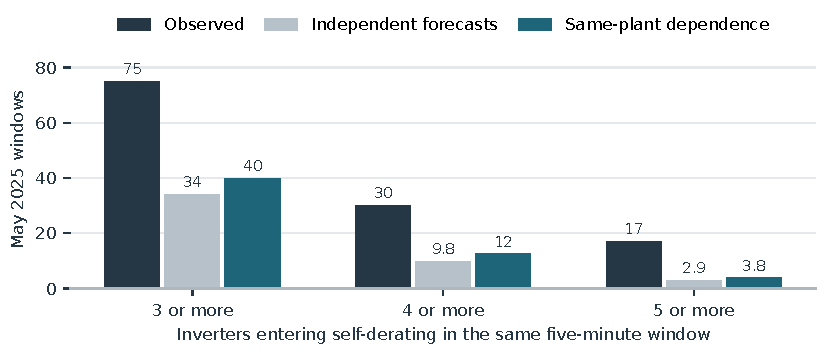
\includegraphics[width=0.84\linewidth]{figures/pv_derating_field.pdf}
\caption*{\textbf{Extended Data Fig. 1. Coincident inverter self-derating in North Macedonia.}
Counts of May 2025 five-minute windows meeting each onset threshold. There were 75 windows with at least three starts, compared with 34 under conditional independence and 40 under a dependence model fitted to January--April records. The two forecasts use the same inverter-level probabilities.}
\end{figure}
\FloatBarrier

\begingroup\small
\begin{thebibliography}{99}
\setlength{\itemsep}{2pt}\setlength{\parsep}{0pt}
\bibitem{golfech} Reuters. \href{https://www.reuters.com/business/energy/edf-shuts-down-golftech-nuclear-plant-due-high-river-temperature-2025-06-30/}{EDF shuts down Golfech nuclear reactor due to high river temperature} (30 June 2025).
\bibitem{hsb} HSB. \href{https://www.munichre.com/content/dam/munichre/hsb/hsb-iic/documents/hsb-energy-insurance-product-sheet.pdf/_jcr_content/renditions/original./hsb-energy-insurance-product-sheet.pdf}{Renewable energy risk solutions}. Operational property product sheet.
\bibitem{chubb} Chubb. \href{https://www.chubb.com/content/dam/chubb-sites/chubb-com/uk-en/business/by-category-construction/documents/pdf/Chubb-UK7377-Construction-Technical_Lines_Brochure-202103.pdf}{Construction and technical lines}. Operational power and business interruption.
\bibitem{dtinsure} Pant, P. et al. Digital-Twin-Based Insurance Risk Differentiation for Photovoltaic Inverter Fleets. Manuscript (2026).
\bibitem{sparc} Pant, P., Tanjavooru, V. T., Hesse, H. \& Hamacher, T. Condition-Aware Multi-Subsystem Reliability-to-Loss Assessment of Utility-Scale Battery Storage Under Claims Scarcity. Manuscript (2026).
\bibitem{aes} Pant, P., Terzija, V. \& Hamacher, T. Actuarial Energy Systems: A Structured Review and Framework for Condition-Informed Insurance. Manuscript (2026).
\bibitem{solarmagix} Daskalov, A. et al. \href{https://doi.org/10.17632/4zgsckxpdy.2}{Dataset for unified photovoltaic-weather multi-station analysis in North Macedonia}. Mendeley Data, v2 (2026).
\bibitem{observed} Pant, P., Terzija, V. \& Hamacher, T. Inverter telemetry reveals clustered derating in a monitored photovoltaic fleet. Research draft (2026).
\bibitem{era5} Copernicus Climate Change Service. \href{https://cds.climate.copernicus.eu/datasets/derived-era5-single-levels-daily-statistics?tab=overview}{ERA5 post-processed daily statistics on single levels}.
\bibitem{heatwave} Pant, P. \href{https://github.com/Prashantgrid/Heatwave}{Heatwave: condition information, adaptation and insurance}. Data and code repository.
\bibitem{allianz} Allianz. \href{https://www.allianz.co.uk/content/dam/onemarketing/azuk/allianzcouk/broker/docs/products/machinery-business-interruption/policy-wordings/mbi-policy-wording-acew1288-18.pdf}{Machinery business interruption policy wording}. Example of a scheduled indemnity period and physical-damage trigger.
\end{thebibliography}
\endgroup

\end{document}
